\documentclass[tikz,convert={size=640,density=300}]{standalone}
\usepackage{amsmath}
\usepackage{amssymb}
\usepackage{pgfplots}
\usepackage{pgfplotstable}
\usetikzlibrary{decorations.pathmorphing}
\usetikzlibrary{arrows}
\usetikzlibrary{calc}
\definecolor{pantone2727}{RGB}{48,127,226}
\definecolor{mymagenta}{RGB}{236,0,140}
\definecolor{myorange}{RGB}{209,115,0}
%\usetikzlibrary{...}% tikz package already loaded by 'tikz' option
\pgfplotsset{compat = newest}

\begin{document}

\def\xmin{-1}
\def\xmax{4}
\def\ymin{-2}
\def\ymax{2}
\def\xnomass{-0.5}
\def\xequil{-2}
\def\xcomp{0}
\def\xstretch{2}

    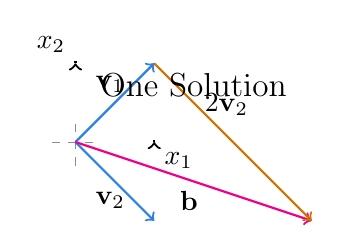
\begin{tikzpicture}[
    spring/.style 2 args={decoration={zigzag, segment length=#1, amplitude=#2},decorate,color=pantone2727},
    coil/.style 2 args={decoration={coil, segment length=#1, amplitude=#2},decorate,color=tulip}
        ]

        \draw[help lines, color=gray!90, dashed] (\xmin - 0.3,\ymin - 0.3) grid (\xmax + 0.3,\ymax + 0.3);
        \draw[->, thick] (\xmin,0)--(\xmax,0) node[below right]{$x_1$};
        \draw[->, thick] (0,\ymin)--(0,\ymax) node[above left]{$x_2$};

        \draw[->,color=pantone2727,thick] (0,0) -- (1,1) node[pos=0.5,above,color=black]{$\mathbf{v}_1\ $};
        \draw[->,color=pantone2727,thick] (0,0) -- (1,-1) node[pos=0.5,below,color=black]{$\mathbf{v}_2\ $};
        \draw[->,color=mymagenta,thick] (0,0) -- (3,-1) node[pos=0.5,below,color=black]{$\mathbf{b}\ $};
        \draw[->,color=myorange,thick] (1,1) -- (3,-1) node[pos=0.4,above,color=black]{\ \,\,$2\mathbf{v}_2$};

        \node[color=black,below] at (1.5,\ymax + 1) {\large One Solution};

    \end{tikzpicture}
\end{document} 